\chapter{Tag Propagation}

So far, our treatment of context networks had made an assumption: context solely consists of events co-occurring with the photo-capture events, and these events are obtained from data sources. The second part of the assumption is not always true in practice. For example, a person's roommate might be a last minute addition to a road trip, who was neither on the email chain or the facebook event, will be ranked very low by the discovery algorithm. A professor whose students are receiving best paper award but was not part of the author list herself might be present at the award ceremony because the conference is being hosted 50 kilometers from her university. Similarly, people at a concert might run into acquaintances because they share the same musical interests. In these cases, the data sources will provide incomplete contextual information which leads the discovery algorithm to rank some candidates poorly.

In this chapter, we will attempt to address this problem of boosting the performance of the CueNet framework by introducing a technique to rank candidates based on their participation profile in previous context networks, personal interests or information. We will present our intuition through a series of examples, and introduce a technique similar to PageRank, which is used to rank pages on the world wide web. In our case, we will rank people in the \texttt{CandidateSet} given set of context networks. Our main differences will lie in the initialization of the score matrix and the propagation of scores \textit{across} the different context networks.

\section{Preliminaries}

Rank propagation techniques have been used to rank nodes in directed graphs. Most commonly seen versions in today's literature are the HITS algorithm invented by Jon Kleinberg \cite{kleinberg1999authoritative} and the PageRank algorithm developed by Larry Page and Sergey Brin \cite{page1999pagerank}. The idea in the latter is to assign a set of initial values to a subset of nodes, and propagate a fraction of these values to their neighbors. Each iteration of the algorithm propagates their scores to the neighboring nodes until the overall ordering of the nodes, according to their scores, does not change. In practice, a few iterations ($<$ 100) on web scale graphs is sufficient to achieve convergence.

\begin{figure}[t]
\centering
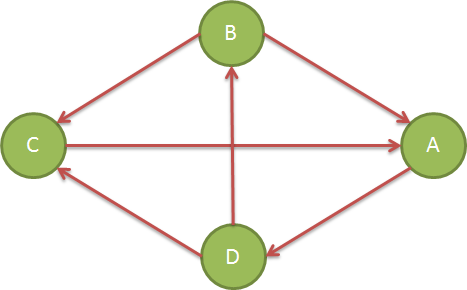
\includegraphics[width=0.65\textwidth]{media/chapter6/pr-example-graph.png}
\caption{Example graph to demonstrate the original Pagerank algorithm.}
\label{fig:pr-graph-example}
\end{figure}

The page rank \cite{page1999pagerank} algorithm, designed to rank large nodes in web graphs is an extension of this idea. The intuition behind page rank is that of the random surfer model. The rank propagation models the behavior of a random web surfer who follows a few links and then gets `bored' and jumps to a random part of the web graph. The final scores of the ranking algorithm converge to the probabilities of such a surfer spending time at a particular page. Another analogy to understand PageRank would be the following: If many surfers (where number of surfers is greater than number of nodes) uniformly choose a page to start surfing from, and move to either one of the outgoing nodes or decide to jump to another page in the graph, then after some iterations, the page rank of a node is fraction of surfers left on it. Mathematically, the page rank of a given web page $i$ at the $k^{th}$ iteration of the rank computation algorithm, denoted as $PR(i, k)$ is defined recursively according to the equation \cite{borodin2001finding}:

\begin{align}
\label{eq:pagerank}
% PR(i) = dD(i) + (1 - d) \sum_{j \rightarrow i} [PR(j)/N(j)] \\  %Equation from Borodin's paper
PR(i, k) = dD(i) + (1 - d) \sum_{j \rightarrow i} [PR(j, k - 1)/N(j)]
\end{align}

In equation \ref{eq:pagerank}, $d$ is the probability with which the random surfer will jump to a sample from the distribution $D(.)$, and with probability (1-d) jumps uniformly at random to one of the pages linked from the current page.

\restylealgo{ruled}
\SetAlgoSkip{}
\begin{algorithm}[t]
\dontprintsemicolon 
\Begin{
  
$R_0$ $\leftarrow$ S  \\
\textbf{loop}: \\
\Indp
  $R_{i+1}$ $\leftarrow$ $AR_i$ \\
  d $\leftarrow$ $||R_i||_1$ - $||R_{i+1}||_1$ \\  
  $R_{i+1}$ $\leftarrow$ $||R_i||_1$ + dE \\
  $\delta$ $\leftarrow$ $||R_{i+1} - R_i||_1$ \\
\Indm
\textbf{while $\delta > \epsilon$}
}
\caption{Original Pagerank Algorithm}
\label{alg:pr-alg}
\end{algorithm}

Let us take a look at how rank propagation works in simple graphs. Consider the directed graph in figure. Let the initial scores of all nodes be 0.25. In the first iteration of the algorithm, if we assume that the surfer will only follow links (i.e., d = 0), the score of node A would be computed as follows. Since A has two incoming edges from B and C, they will transfer a portion of their scores to A. Since B has two outgoing edges, it will transfer half of its score to A. C has only one outgoing edge, and therefore transfers all of its score to A. Thus, the value $PR(A)$ becomes $0.25/2 + .25 = 0.375$ at the end of the first iteration. Similarly, B obtains half the score of D; C obtains half of B and half of D; and D obtains the full score of A. For each node, we can rewrite \ref{eq:pagerank} as follows:

\begin{flalign}
\label{eq:p1}
&PR(A, i) = \frac{PR(B, i-1)}{2} + PR(C, i-1) & \\
&PR(B, i) = \frac{PR(D, i-1)}{2} & \\
&PR(C, i) = \frac{PR(D, i-1)}{2} + \frac{PR(B, i-1)}{2}& \\
&PR(D, i) = PR(A, i-1) & 
\end{flalign}

If the probability of jumping to a web page from the distribution D is 0.15, and we assume that the probabilities in $D$ are equally likely, the above equation to compute the new pagerank of node A becomes $PR(A, i) = \frac{d}{N} + (1-d)\frac{PR(B, i-1)}{2} + PR(C, i-1) = 0.35625$. Table \ref{tbl:prc} shows the different values of page rank for each node in our example graph per iteration until it converges. We assume that the initial ranks of each node is 0.25. The difference in ranks is computed using L1 norm of the difference of ranks in the current and previous iteration.

\begin{flalign}
\label{eq:norm}
\delta = \sum_{\forall i}{|PR(i)  - PR(i-1)|}
\end{flalign}

\begin{table}[h]
\begin{center}
\begin{tabular}{ |c|c|c|c|c|c| }
  \hline
  \texttt{k} & \texttt{A} & \texttt{B} & \texttt{C} & \texttt{D} & \texttt{$\delta$}\\
  \hline
  1  &  0.25000  &  0.25000  &  0.25000  &  0.25000  &  - \\
  1  &  0.35625  &  0.14375  &  0.25000  &  0.25000  &  0.21250 \\
  2  &  0.31109  &  0.14375  &  0.20484  &  0.34031  &  0.18062 \\
  3  &  0.27271  &  0.18213  &  0.24323  &  0.30193  &  0.15353 \\
  4  &  0.32165  &  0.16582  &  0.24323  &  0.26930  &  0.09788 \\
  5  &  0.31472  &  0.15195  &  0.22243  &  0.31090  &  0.08319 \\
  6  &  0.29114  &  0.16963  &  0.23421  &  0.30501  &  0.05893 \\
  7  &  0.30868  &  0.16713  &  0.23922  &  0.28497  &  0.04508 \\
  8  &  0.31187  &  0.15861  &  0.22964  &  0.29987  &  0.03619 \\
  9  &  0.30011  &  0.16495  &  0.23236  &  0.30259  &  0.02352 \\
  10 &  0.30511  &  0.16610  &  0.23620  &  0.29259  &  0.02000 \\
  ... &  ...  &  ...  &  ...  &  ...  &  ... \\
  34 &  0.30554  &  0.16381  &  0.23343  &  0.29721  &  0.00002 \\
  35 &  0.30554  &  0.16382  &  0.23344  &  0.29721  &  0.00002 \\
  36 &  0.30554  &  0.16381  &  0.23344  &  0.29721  &  0.00001 \\
  37 &  0.30554  &  0.16381  &  0.23343  &  0.29721  &  0.00001 \\
  38 &  0.30554  &  0.16381  &  0.23344  &  0.29721  &  0.00001 \\
  39 &  0.30554  &  0.16381  &  0.23344  &  0.29721  &  0.00000 \\
  40 &  0.30554  &  0.16381  &  0.23343  &  0.29721  &  0.00000 \\
  \hline
\end{tabular}
\caption{Page rank scores for nodes in the example graph per iteration.}
\label{tbl:prc}
\end{center}
\end{table}

The page rank algorithm is shown in algorithm \ref{alg:pr-alg}. R is a vector over all the nodes in the graph. A is an adjacency matrix where each cell measures is the reciprocal of outgoing edge count. If $u$ and $v$ are two nodes, and there are $N_u$ outgoing edges from $u$ and one of them ends in $v$, then $A(u, v) = 1/N_u$. The expression $||R||_1$ is the L1 or Manhattan norm of a vector $R$, which is computed as $\sum_{\forall i} |R_i|$. The vector $S$ is the initial score assigned to the nodes. On a large scale, pagerank scores are computed using the MapReduce framework \cite{dean2008mapreduce}. Each iteration of the computation corresponds to one map reduce job. Multiple such iterations are performed to obtain the final results.

\section{Intuition}

To rank objects in context networks, we modify the random surfer model slightly to model the movement of objects between different networks. Consider a set of context networks, each of which correspond to a \texttt{photo-capture-event}. Each network consists of a set of participating objects. An object in a particular network can move to a neighboring context network depending on the differences between properties of the two networks. If the two photos were captured right next to each other, and contain very similar types of events, and object instances, then there is a high probability that this person who was tagged in one of them, will be present in the other. Time is one such axis of propagation. Other properties such as event class, object co-occurrence, place (type of place or the distance) of event occurrence or subevent patterns in context network can provide different axes to propagate tags between photos.

\begin{figure}[t]
\centering
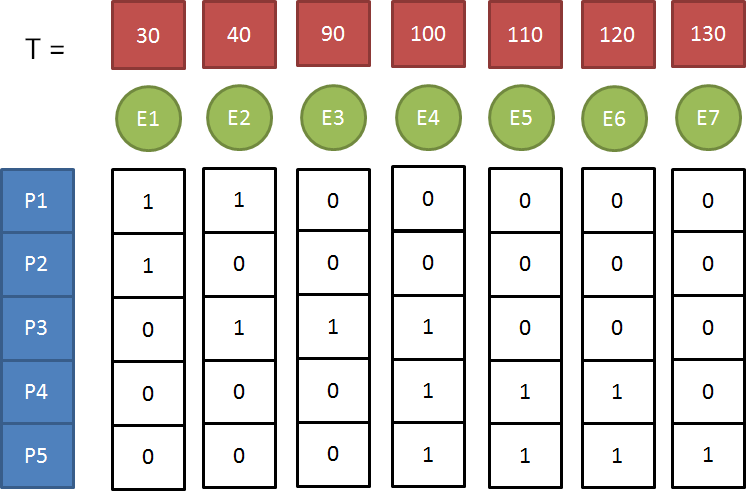
\includegraphics[width=0.65\textwidth]{media/chapter6/time-example-2.png}
\caption{Propagating values through temporal relations.}
\label{fig:time-example}
\end{figure}

Consider the context networks shown in figure \ref{fig:time-example}. Events \texttt{E1} - \texttt{E7} contain one or more persons from the candidate set \texttt{P1} - \texttt{P5}. The binary vector below event describes whether an object was present in the event or not. \texttt{P1}, for example, participates in \texttt{E1} and \texttt{E2}. \texttt{P5} participates in events \texttt{E4} through \texttt{E7}. The top row shows the time of occurrence for all events. We shall assume that other properties of an event (class, location and subevent structure) are same, and therefore do not effect the propagation. Since \texttt{E6} contains \texttt{P4}, it can be said that there is a higer chance of \texttt{P4} participating in \texttt{E7} than in \texttt{E1} for two reasons. First, the object distribution in \texttt{E1} is very different from \texttt{E6}. \texttt{P4} has never participated in any event with the \texttt{P1} and \texttt{P2}. Second, because the temporal difference is much higher, very little can be estimated about the presence of a person in an event. If we quantify the object similarity using a set similarity measure, such as the jaccard index (represented by $d_s(e_i, e_j)$, and the effect of time using a formula $1 - \frac{\Delta T}{T_{max}}$, where $\Delta T$ is the difference between occurrence times of two events in question, represented as $d_t(e_i, e_j)$, then we can say that the score of a person will appear in some Ex at the $i^{th}$ iteration, $M(Ex, p, i)$, who is known to have appeared in some other set of events $\mathcal{E}$, where $Ex \notin \mathcal{E}$ is:

\begin{align}
\label{eq:puirank}
M(Ex, p, i) \leftarrow \sum_{e \in \mathcal{E}}[ d_t (e, Ex) d_s (e, Ex) M(e, p, i-1) ]
\end{align}

Similarly, look at figure \ref{fig:location-example} where the context networks now differ in type and location of occurrence as well. We show the event class information (indicated by `C') and location information with `L' of the event above the nodes. Their timestamps are as before, but our original assumption about spatial and ontological consistency no longer holds. Here, can we need to exploit some ontological properties about event similarities to propagate scores. If we know that \texttt{L1} is a \texttt{conference}, \texttt{L2} is a \texttt{music-event} and \texttt{L3} is a party, then can we say that \texttt{L2} events are more likely to contain the untagged person than the \texttt{conference} events. Likewise, spatial relationships propagate higher scores to individuals between events which occur near each other, than those which occur further away.

\begin{figure}[h]
\centering
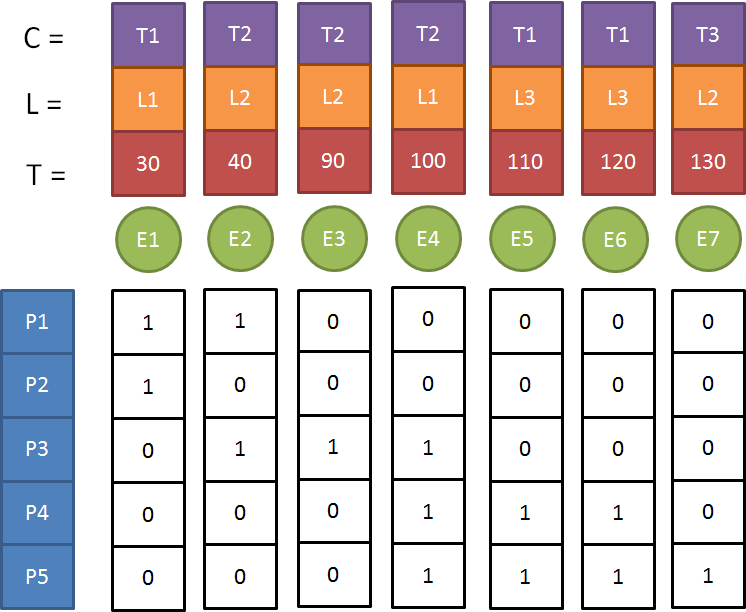
\includegraphics[width=0.65\textwidth]{media/chapter6/multi-property-example.png}
\caption{Other properties of events (space, type, subevent hierarchy patterns or object co-occurrence could be used to propagate scores.}
\label{fig:location-example}
\end{figure}

In this chapter, we will modify the page rank technique (algorithm \ref{alg:pr-alg}) to rank entities on a given set of context networks, to determine who might be participating in a new events. We will initialize scores of the nodes on the basis of what is known about the new event: the type of the instantiating class, the participating objects, and propagate the scores based on a set of propagation functions which we will introduce in the next section. Since the basic propagation algorithm is an expensive one, we will look at some ways to reduce the size of the context networks, so the algorithm converges quickly, and still provides useful results.

\section{Rank Propagation in Context Networks}

In order to rank candidates for a new given photo, we go by the observation that people participate in similar kinds of types, and spend time with similar groups of people. In other words, the distribution of people in events is not random. By ranking events, we are ordering them by some metric of similarity with respect to the context network containing the new photo. Events encapsulate heterogeneous information. Thus, their similarities must be computed across the different kinds of entities they encapsulate. For example, two event instances of the same class which have no common participating object are less similar to each other than two others which are of the same type and contain same participating objects.

For our application of face tagging, computing similar similarities across time, space, type and object information of events. In order to formalize our rank propagation mechanism, we introduce the concept of a propagation function. A propagation function will transfer score from one object in a event to itself in another event through specific property of the event. For example, if we can design a propagation algorithm around two \texttt{temporal} and \texttt{spatial} properties, scores will be transferred based only on the temporal and spatial attribute values of the events respectively. We say that the propagation function contributes a \textit{transfer ratio} across an axis. We follow the steps as shwon in algorithm \ref{alg:pr-alg} with the following differences: \textbf{First}, the vector $S$ is setup based on the distribution of persons present and the attributes of the events in the new context networks. \textbf{Second}, the matrix $A$ is computed as the product of all the transfer ratios between two events. For two events, $u$ and $w$, and propagation functions $P_t$ and $P_s$ (temporal and spatial propagations), the propagation vector is $V$ = $[P_t, P_s]$, and the score transfer vector from $u$ to $w$, $V(u, w)$ = $[P_t(u, w), P_s(u, w)]$ and the value $A(u, w)$ = $\mathcal{C} \times P_t(u, w) \times P_s(u, w)$, where $\mathcal C$ is a constant scaling factor.

\subsection{Propagation Functions}

In this section we introduce the propagation functions used in our work to rank events for the face tagging application.

\begin{itemize}
\item \textbf{Temporal Propagation}: For events $u$ and $w$, the temporal propagation function $P_t (u, w)$ propagates a fraction of the score of node $u$ to $w$ proportional to the difference between \texttt{u.duration} and \texttt{v.duration}. The transfer function can be modeled using uniform gaussian or zipf distributions. The advantage with such distributions is to model high transfer of scores who occur nearby in the temporal dimension, and ignoring those which happened too far away. The distribution parameters will be constant and set by the designer.

\item \textbf{Spatial Propagation}: Similar to the temporal propagation function, this takes into consider the spatial attributes of an event while transferring scores. The distance between two coordinates can be computed through one of three ways. First, a table based scheme which allots scores based on the address information of the event. Here, high scores are given if the two events occur in the same city in comparison to those within the same country. Second, using euclidean distance between GPS coordinates of the two events. Third, compute the actual `as the crow flies' distance between the two locations. We use the formula based on the spherical law of cosines: where the distance between two pair of coordinates d(lat1, lon1, lon2), is given by (where $\mathcal R$ is the radius of the Earth (6378 kms)):


\begin{align}
\label{eq:distance}
\mathcal R \arccos(\sin(lat1) \sin(lat2) + \cos(lat1) \cos(lat2) \cos(lon2 - lon1))
\end{align}


\item \textbf{Type Propagation}: The class of the event instance is taken into consideration to compare two events. We use the concept of ontological distance to compute the type propagation score transfer. We extend the concept of \texttt{Is-A} distance given in \cite{ranwez2006ontological}. For given a subsumption hierarchy, $a$ is an ancestor of $b$ iff there is a path between $a$ and $b$. The set of concepts having a as ancestor is denoted by $desc(a)$, while its ancestors are denoted as $ansc(a)$. The set of exclusive ancestors (if a node is an ancestor of exactly one of the two nodes) of $a$ and $b$ is denoted by $exAnsc(a, b)$. The subsumption ontological distance is defined as:

$d_{IS}(a, b) = |desc(exAnsc(a, b)) \cup desc(a) \cup desc(b) - desc(a) \cap desc(b)|$.

Events also exhibit subevent relationships. Two events could have very common subevents, but might have significant subsumption distance. In this case, we want to reduce this distance. We introduce the subevent distance as the number of common subevents as the number of common descendant in the subevent hierarchy of the ontology. For a node $a$, $subdesc(a)$ is the set of all $a$'s subevents and their transitive descendants.

$d_{SE}(a, b) = |subdesc(a) \cap subdesc(b)|$

Our ontology distance is the sum of subsumption distance and the subevent distance. This number can be normalized with the number of perdurant classes present in the ontology.

$d(a, b) = D_{IS}(a, b) + D_{SE}(a, b)$

\item \textbf{Object Propagation}: If two events have the same set of participating objects, then the score transfered through object propagation is very high. If they have no common objects, then this transfer would be 0. We use Jacquard index to compute this ratio. For two sets of objects $A$ and $B$, the jacquard index is computed as:
\begin{equation}
J(A, B) = \frac{A \cap B}{A \cup B} \nonumber
\end{equation}

\item \textbf{Structural Propagation}: The last propagation function we use is the propagation from an event to its instance subevents. Here we use a function which is similar to the one used in pagerank while computing the transfer from a graph node through an outgoing edge. If event $B$ is a subevent of $A$ (we can use the web graph as an analogy where the subevent edge is an outgoing edge from $A$ to $B$), and $A$ has $n$ subevents, then the propagation ratio from $A$ to $B$ is $1/n$.

\end{itemize}

\section {Propagation Algorithm}

The final transfer ratio is the product of all the individual transfer ratios. This allows us to transfer smaller scores if the two events differ largely in any one attribute. This is particularly useful when many events occur spatiotemporally close to each other, but are instances of very different event classes. On the other hand, a sum based combination of the individual scores would propagate larger number of individuals because there is atleast one good axis.

We will compute the scores of objects using the following steps. Construct a map $M$, such that $M(V, o) = 1$, if the object $o$ was participating in $V$. Let $\mathcal P = \{P_1, P_2 $ ... $ P_n\}$ be the set of all propagation functions. The score transfer, $\Delta(x, y, o)$ for the object $o$ from a node $x$ to $y$ is given by the equation: $\prod_{1 \leq i \leq n} P_i(x, y) M(x, o, i-1)$. The score at the end of iteration $i$ for $o$ is given as the sum of all $\Delta(x, \bar{y}, o)$, where $ \bar{y} \in \bar{Y}$. $\bar{Y}$ is the set of all nodes which are within satisfy the filter function $F$, such that $F(x, \bar{y}) = true$. This function is used to limit the number of propagations between events. Unlike the web graph where each nodes points to a very tiny fraction of web pages, propagation between events is $O(|V|^2)$ where $|V|$ is the number of events per iteration. If the score of an object is 1, then we do not update its score (the object is known to be present in the event). We call such entries in the map as immutable entries. For every mutable entry, the final score of o at the end of iteration i computed as:

\begin{equation}
M(V, o, i) = \frac{\sum_{y \in \bar{Y}} \prod_{1 \leq i \leq n} P_i(y, V) M(y, o, i-1)}{|\bar{Y}|}
\end{equation}

We compute $\delta(V)$ as the difference between object scores of the event $V$ between two iterations, using L1 norm (similar to the procedure in algorithm \ref{alg:pr-alg}). The biggest difference in propagation is denoted by $\delta = max(\delta(V_1), \delta(V_2), ... )$. The iterative score computation is continued until $\delta < \epsilon$, a very small constant. At this point, the scores in each event are checked, and the objects with highest scores in each event are considered to be the next best guess. These objects can be verified using a face verification algorithm or manually. If they indeed exist, the score for this object must be updated to 1 in the $M$ map and its entry made immutable. 

\section{Experiments}

\begin{figure}[t]
\begin{minipage}[b]{0.5\linewidth}
\centering
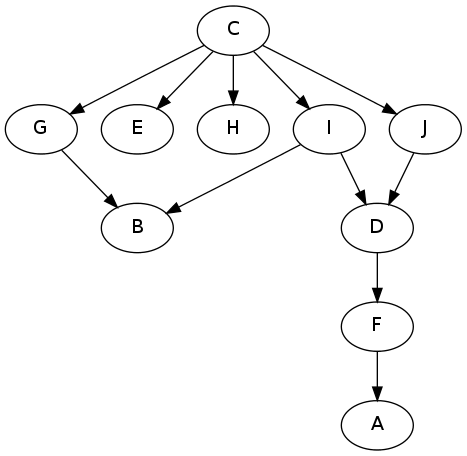
\includegraphics[width=0.7\textwidth]{media/chapter6/sample-ontology.png}
\caption{Example of a subsumption hierarchy created as part of the ontology generation process.}
\label{fig:sample-ontology}
\end{minipage}
\hspace{0.5cm}
\begin{minipage}[b]{0.45\linewidth}

\begin{tabular}{ |c|c|c|c|c|c|c|c|c|c|c| }
  \hline
  & \texttt{A} & \texttt{B} & \texttt{C} & \texttt{D} & \texttt{E} & \texttt{F} & \texttt{G} & \texttt{H} & \texttt{I} & \texttt{J} \\
  \hline
    \texttt{A}  &  0  &  6  &  9  &  2  &  7  &  1  &  7  &  7  &  5  &  5 \\
    \texttt{B}  &  6  &  0  &  9  &  6  &  7  &  6  &  5  &  7  &  5  &  7 \\
    \texttt{C}  &  9  &  9  &  0  &  7  &  9  &  8  &  8  &  9  &  5  &  6 \\
    \texttt{D}  &  2  &  6  &  7  &  0  &  7  &  1  &  7  &  7  &  3  &  3 \\
    \texttt{E}  &  7  &  7  &  9  &  7  &  0  &  7  &  3  &  2  &  6  &  5 \\
    \texttt{F}  &  1  &  6  &  8  &  1  &  7  &  0  &  7  &  7  &  4  &  4 \\
    \texttt{G}  &  7  &  5  &  8  &  7  &  3  &  7  &  0  &  3  &  5  &  6 \\
    \texttt{H}  &  7  &  7  &  9  &  7  &  2  &  7  &  3  &  0  &  6  &  5 \\
    \texttt{I}  &  5  &  5  &  5  &  3  &  6  &  4  &  5  &  6  &  0  &  3 \\
    \texttt{J}  &  5  &  7  &  6  &  3  &  5  &  4  &  6  &  5  &  3  &  0 \\
  \hline
\end{tabular}
\caption{The \texttt{is-A} distance matrix for classes in figure \ref{fig:sample-ontology}.}
\label{tbl:semantic-distance}
\end{minipage}
\end{figure}

We investigate the convergence behavior of our propagation algorithm. To simulate this experiment, we use the generative model described in section \ref{section:generative_models}. We generate an ontology using the following steps: A random number of entities are chosen, and a subsumption hierarchy is created (similar to the one shown in \ref{fig:sample-ontology}). A fraction of these events are assigned a subevent hierarchy, which uses the step described in section \ref{section:generative_models}. For this experiment we restrict the depth of the subevent hierarchy to be 2, and each event class to contain atmost 3 subevents. Events are instantiated randomly. If the ontology specifies a subevent structure, we instantiate subevents too. For each subevent class we use a uniform random generator to decide if it should be instantiated or not. We generate 1000 events for this experiment. It must be noted that this is a fairly large number as we are propagating scores for each event to all the others one due to temporal and spatial propagations. Thus, for 1000 events, we expect a million propagations per iteration. We use a linear distribution for spatial and temporal propagation functions. For the temporal function, this means that the propagation decreases linearly until 5\% of the total timespan of the events, beyond which point no score is transferred. Similarly spatial propagation decreases 10\% of the maximum distance between two event instances in the dataset (these percentages were arbitrarily chosen).

\begin{figure}[h!]
\centering
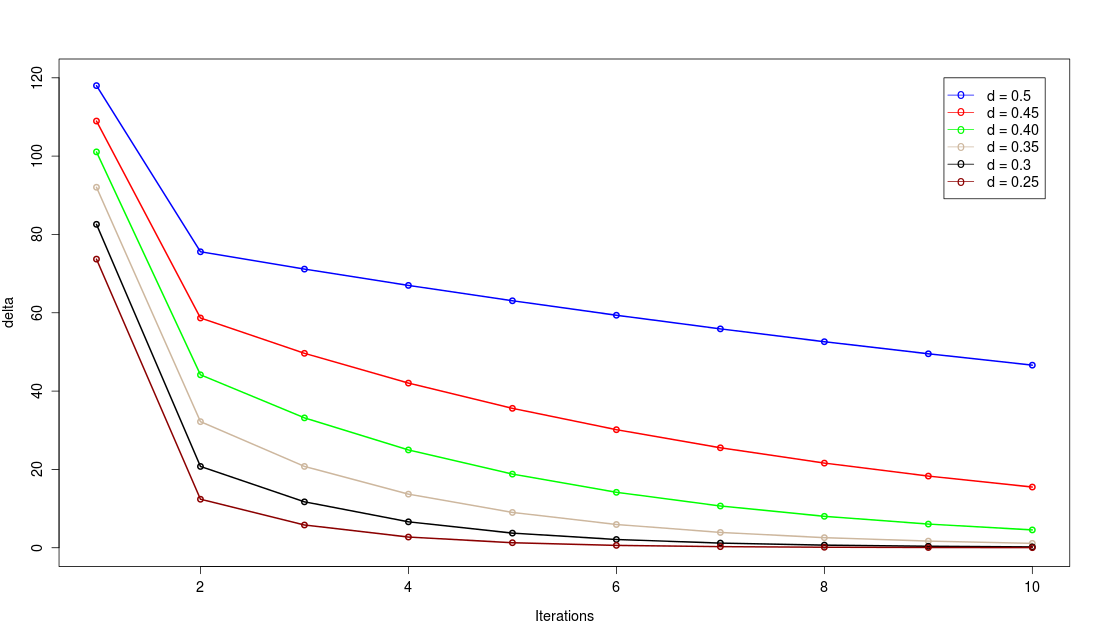
\includegraphics[width=0.85\textwidth]{media/chapter6/convergences.png}
\caption{Rate of convergence of the propagation algorithm for varying values of $d$.}
\label{fig:convergences}
\end{figure}

Figure \ref{fig:convergences} plots the L1 norm in the rank vector for different values of the decay factor per iteration. For a higher value of the decay factor, $d$, we see a faster convergence rate. It must be noted that for this convergence is achieved within a few iterations. We also plot the rate of convergence for datasets with different number of instances. In figure \ref{fig:convergences-inreasing-nodes}, we plot the decreasing value of $\delta$ on a log scale for two datasets, one containing 1000 nodes, and the other with 1500 nodes. The plot shows the increasing number of iterations for larger datasets to converge to the same value.

\begin{figure}[h]
\centering
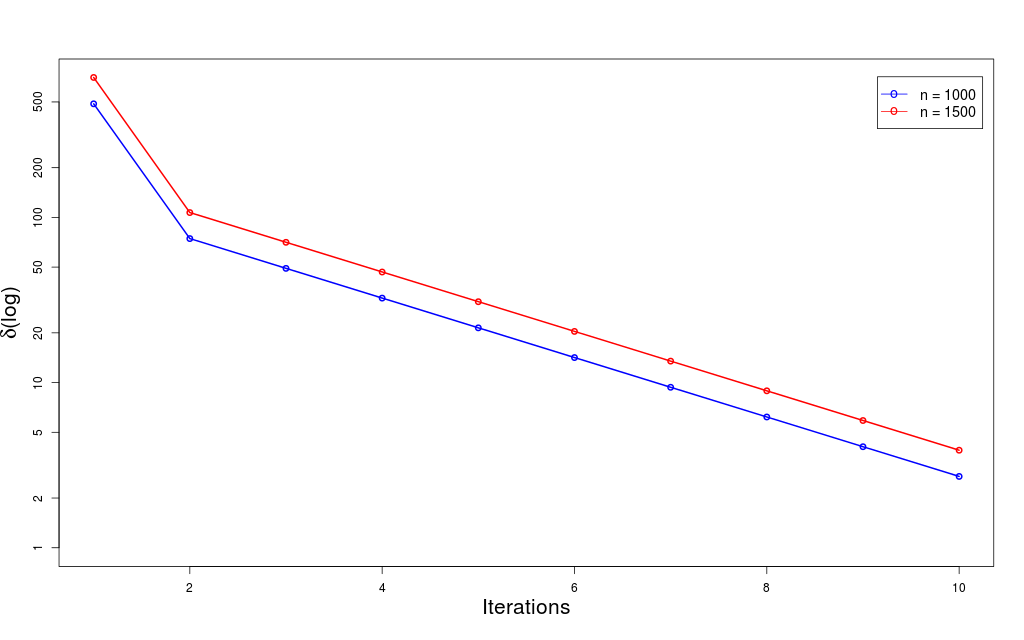
\includegraphics[width=0.85\textwidth]{media/chapter6/convergence-with-node-change.png}
\caption{Rate of convergence with increasing number of instances, for $d$ = 0.85.}
\label{fig:convergences-inreasing-nodes}
\end{figure}

Now, we shall apply this technique to ranking real-world photos. We consider a dataset containing 120 photos taken during a \texttt{social-party} event. All photos were annotated by the owner, and contain required EXIF tags. In order to test the algorithm, we construct context networks for all photos (using the ground truth information supplied by the user). We select some photos randomly, and remove all object information from them. The propagation algorithm is used to order the collection of objects for these photos. We use precision and recall to analyze the performance of the propagation algorithm. For this experiment, we only use temporal propagation with a linear transfer function which decreases linearly until 2\% of the timespan. In figures \ref{fig:good} - \ref{fig:poor}, we see different precision recall graphs drawn for different photos. The performance for ranking people in a photo can vary because of many reasons. In our experiments, we see that many personal photos contain the same set of people in sequence. This is because the photographer was capturing a specific event where these people were playing a prominent role or the photographer was not satisfied with the aesthetic quality of photo, and tried multiple captures before settling on a photo. In such cases, we see all the objects in the ground truth rank very highly from the propagation algorithm. Figure \ref{fig:good} shows the precision recall graph for two such photos. On the other extreme, the algorithm fares poorly when new people are introduced in the photo. Here, they are ranked very low as the expected people are those who were captured in nearby photos. This can be seen in the figure \ref{fig:poor}. A set of photos also displayed intermediate results (figure \ref{fig:average}), where some of the entities ranked highly but the rest were ranked very low. The distribution of people in these photos looked such that some people were present in nearby photos, but others were not. This is due to the nature of the event. Since our linear propagation function does not model the behavior of photographers in such \texttt{party} events, the algorithm sees seemingly random behavior. What is actually happening is that the photographer moves his vantage between groups of people in the party. If the propagation model can be extended to capture this event specific behavior, we can possibly boost the performance of such an algorithm. 

\begin{figure}[t]

\begin{minipage}[b]{0.5\linewidth}
\centering
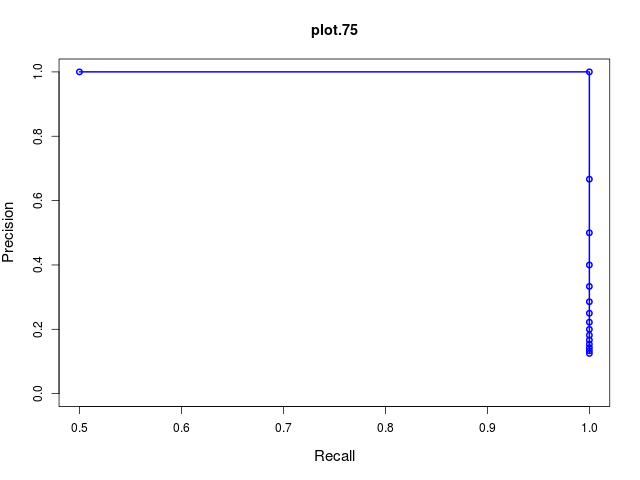
\includegraphics[width=\textwidth]{media/chapter6/pr-graphs/plot-75.png}

\end{minipage}
\hspace{0.5cm}
\begin{minipage}[b]{0.5\linewidth}
\centering
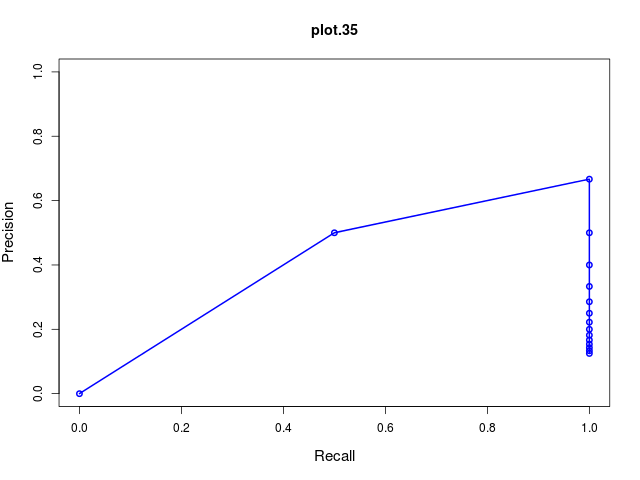
\includegraphics[width=\textwidth]{media/chapter6/pr-graphs/plot-35.png}
\end{minipage}
\caption{Photos where people were ranked very high.}
\label{fig:good}

\begin{minipage}[b]{0.5\linewidth}
\centering
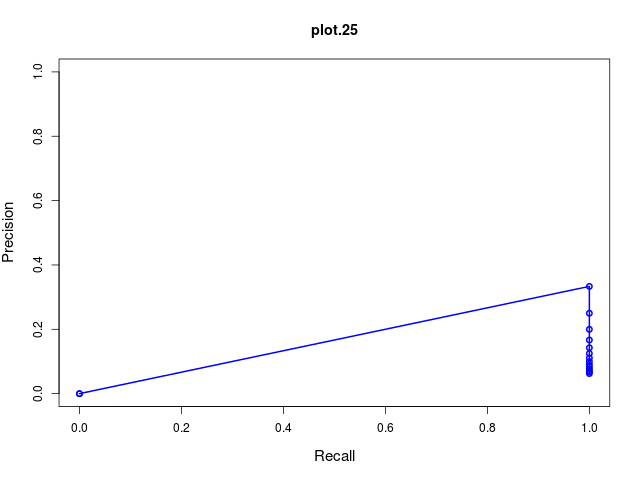
\includegraphics[width=\textwidth]{media/chapter6/pr-graphs/plot-25.png}
\end{minipage}
\hspace{0.5cm}
\begin{minipage}[b]{0.5\linewidth}
\centering
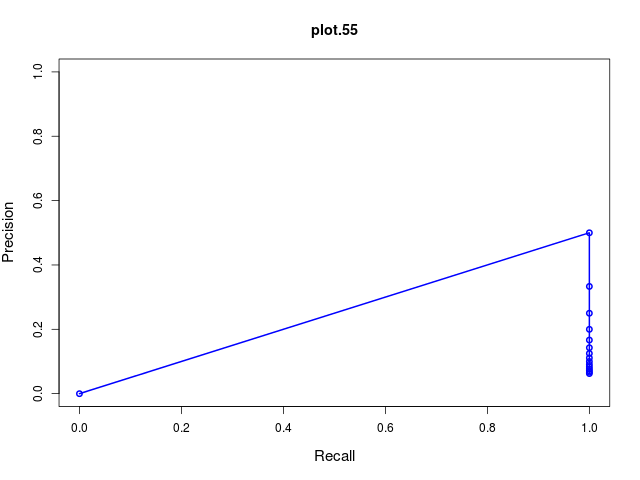
\includegraphics[width=\textwidth]{media/chapter6/pr-graphs/plot-55.png}
\end{minipage}
\caption{Photos where `random' distribution of people were seen.}
\label{fig:average}

\begin{minipage}[b]{0.5\linewidth}
\centering
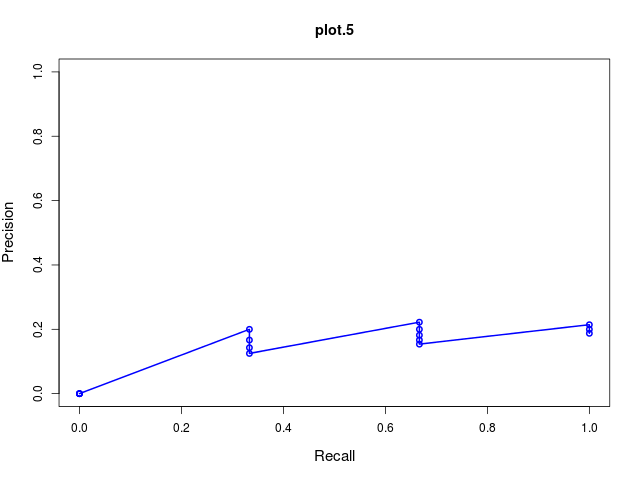
\includegraphics[width=\textwidth]{media/chapter6/pr-graphs/plot-5.png}
\end{minipage}
\hspace{0.5cm}
\begin{minipage}[b]{0.5\linewidth}
\centering
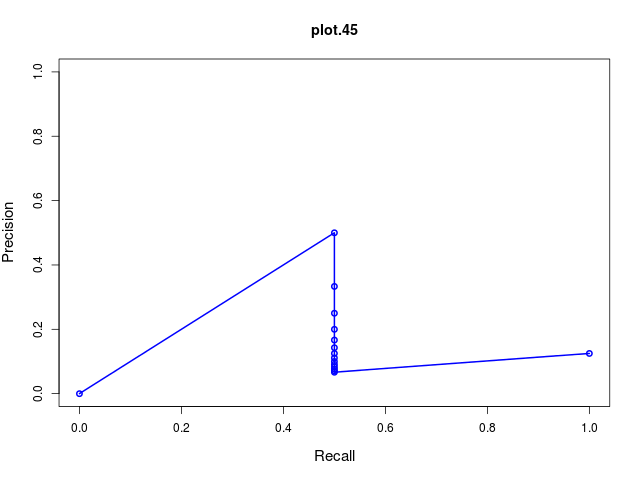
\includegraphics[width=\textwidth]{media/chapter6/pr-graphs/plot-45.png}
\end{minipage}
\caption{Photos where people were ranked poorly because they were not present in nearby photos.}
\label{fig:poor}

\end{figure}

\section{Conclusion}
In this chapter, we outlined a technique similar to \cite{page1999pagerank} to order the entities when only partial contextual information for a photo is available. There are two main advantages to such a technique. First, it can be used to tag photos which are captured after an event's duration has passed. Since the people are still participating in event, after its scheduled duration has passed, the photos taken during this interval would have \textit{missed} the contextual information available from different sources. In such cases, the tagged people from the previous photos can be propagated to these photos. Second, during long term events like conferences people will participate in different types of events such as trips to landmarks, dinner with colleagues or visit friends in the city where the conference is occurring. 

Our ontological distance measures take care of some of these cases, but there are many opportunities to explore and determine good ways of model people's behavior to propagate their scores across the different events. One way is to explicitly model such individual behavior using ontologies or similar tools. This will require many experts to work hands-on to tailor such models. On the other hand, appropriate data driven machine learning tools could be used to learn the behavior from a training set of photos, and apply them to propagate scores in a testing set. This technique requires a large amount of user data to train efficient models. But requires fewer experts to curate the models. Alternatively, a hybrid method can be devised, which utilizes the strength of both techniques, and achieves reasonable results.